\parindent0pt{\Large{\textcolor{red}{Dieses Kapitel ist noch nicht offiziell Bestandteil des Testat 2.}}}
\section{Feinkonzept}
	Nach der Entscheidung für ein Grobkonzept folgt nun die Detaillierung dieses Konzeptes in ein Feinkonzept. Die ursprünglich sieben Teilprobleme wurden in 19 Subteilprobleme auf gesplittet. Zu all diesen Subteilproblemen existieren wiederum Lösungsvarianten, die in Abbildung \ref{abb:Feinkonzept} dargestellt sind.
	
	\begin{figure}[h!]
		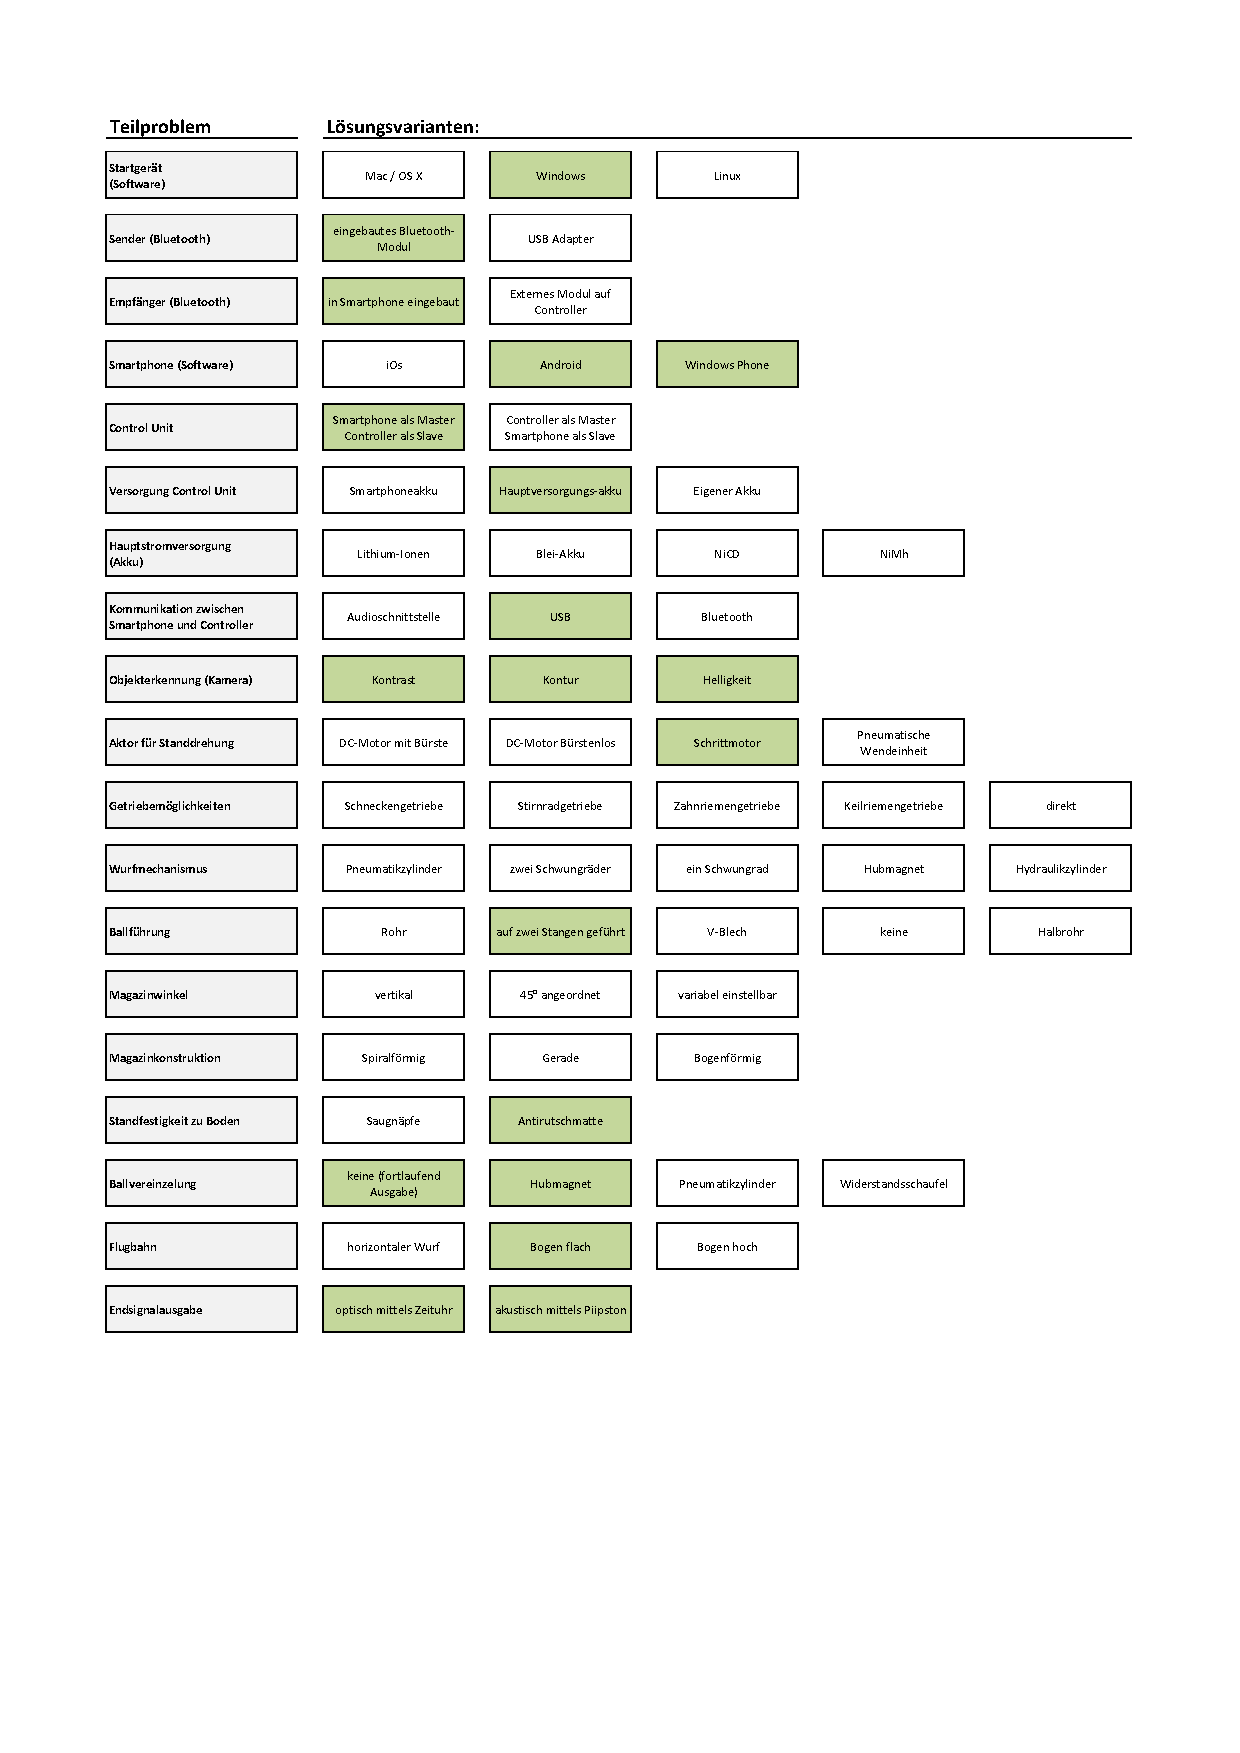
\includegraphics[page=1,scale=0.77,clip,trim=17mm 70mm 18mm 20mm]{Morphologie/Bilder/Feinkonzept.pdf}
		\centering
		\caption{Feinkonzept}
		\label{abb:Feinkonzept} 
	\end{figure}
	
	Die grün eingefärbten Lösungsvarianten in Abbildung \ref{abb:Feinkonzept} stellen unsere Entscheidung im jeweiligen Subteilproblem dar. Nachfolgend ist eine Erklärung zur Lösungsfindung zu jedem einzelnen Subteilproblem beschrieben.\\
	\\	
	\textbf{Startgerät (Software})\\
	Als Startgerät wird ein Notebook mit dem Windows-Betriebssystem verwendet, da es ein viel verbreitetes, stabiles, gut dokumentiertes Betriebssystem ist und alle nötigen Funktionen zur Ausführung unserer Problemstellung hat. Keines der Teammitglieder verwendet ein Notebook mit Mac/OSX oder Linux, diese beiden Betriebssysteme kommen daher nicht in Frage.\\
	\\
	\textbf{Sender (Bluetooth)}\\
	Das eingesetzte Notebook hat ein eingebautes Bluetooth-Modul welches als Sender verwendet werden kann, daher wird ein USB-Bluetooth-Adapter überflüssig.\\
	\\
	\textbf{Empfänger (Bluetooth)}\\
	Als Empfänger auf der Seite des Ballwerfers wird das im Smartphone integrierte Bluetooth-Modul verwendet. Das Smartphone agiert in diesem System als Master, der Controller übernimmt die Rolle des Slaves.\\
	\\
	\textbf{Smartphone (Software)}\\
	Beim Smartphone-Betriebssystem kommen nur die Open source Variante Android und das Windows-Phone-Betriebssystem in Frage, da sie bezüglich Zugriff auf die vorhandenen Schnittstellen nicht eingeschränkt sind. Eine genaue Festlegung ist zurzeit noch nicht möglich. Definitiv ausgeschlossen ist das iOS Betriebssystem von Apple, da keine Programmiererfahrung auf diesem Gebiet vorhanden ist und der Zugriff auf die nötigen Schnittstellen eingeschränkt ist.\\
	\\
	\textbf{Versorgung Control-Unit}\\
	Der Hauptversorgungsakkumulator soll die Versorgung der Control-Unit übernehmen.\\
	\\
	\textbf{Hauptstromversorgung (Akkumulator)}\\
	Die Art des Hauptversorgungsakkumulators wird erst mit der Konstruktion und Dimension des Produkts klar, bleibt im daher im Moment noch offen.\\
	\\
	\textbf{Kommunikation zwischen Smartphone und Controller}\\
	Die Kommunikation des Smartphones zum Controller findet via USB-Kabel statt. Dies Aufgrund der Controller-Wahl, der unter anderem die Kommunikation mit USB zulässt.\\
	\\
	\textbf{Objekterkennung (Kamera)}\\
	Bei der Objekterkennung mittels Kamera werden idealerweise alle drei optischen Bestimmungskriterien Kontrast, Helligkeit und Kontur zur Objektidentifikation verwendet. Falls die Erkennung mittels Kamera nicht realisierbar ist, stellt Ortung via Ultraschall eine interessante Alternative dar.\\
	\\
	\textbf{Aktor für Standdrehung}\\
	Die Drehung der Plattform erfolgt direkt durch einen Schrittmotor, da diese Lösung kleine Veränderungen des Winkels zulässt und in gleichmässigen Schritten gesteuert werden kann.\\
	\\
	\textbf{Getriebemöglichkeiten}\\
	Ob Getriebemöglichkeiten zum Einsatz kommen, ist durch den momentanen Stand des Produkts nicht gegeben.\\
	\\
	\textbf{Wurfmechanismus}\\
	Der Pneumatikzylinder erlaubt eine hohe Wurfreproduzierbarkeit. Mithilfe zweier Schwungräder kann durch einbringen eines Dralls die Flugbahn stabilisiert werden. Bei nur einem Schwungrad besteht der Vorteil, dass nur ein Motor verwendet werden muss. Ein Hubmagnet bietet eine gute Alternative zur Pneumatik-Ausführung, da keine externe Druckluft-Versorgung nötig ist. Der Hydraulikzylinder fällt aufgrund der niedrigen Geschwindigkeit weg. Die genaue Auswahl des Wurfmechanismus wird durch die Testbauten ermittelt.\\
	\\
	\textbf{Ballführung}\\
	Die Ausführung auf zwei oder mehr Stangen ist bauleicht und hat wenig Laufwiederstand für den Ball. In einem geschlossenen und halboffenen Rohr ist die Gefahr von Verstopfungen und Laufreibungen der Bälle höher als bei einer Lösung mittels Stangen.\\
	\\
	\textbf{Magazinwinkel und Magazinkonstruktion}\\
	Der Magazinwinkel und Magazinkonstruktion kann erst im Zusammenhang mit der Gesamtlösung respektive des Wurfmechanismus erarbeitet werden.\\
	\\
	\textbf{Standfestigkeit zu Boden}\\
	Die Standfestigkeit soll mittels Antirutschmatte gewährleistet werden, falls dies nicht genügt, können Saugnäpfe verwendet werden.\\
	\\
	\textbf{Ballvereinzelung}\\
	Falls es die Umstände zulassen, wird auf eine Ballvereinzelung verzichtet, wenn sie aber aufgrund des Wurfmechanismus nötig wird, soll ein Hubmagnet als Schieber zum Einsatz kommen.\\
	\\
	\textbf{Flugbahn}\\
	Die Flugbahn soll in einem flachen Bogen erfolgen, um das Gerät mit einen möglichst tiefen Schwerpunkt auszustatten und dass der Ball nicht aus dem Korb zurückspringen kann.\\
	\\
	\textbf{Endsignalausgabe}\\
	Die akustische und optische Endsignalausgabe erfolgt laut Aufgabenstellung auf dem Startgerät (Notebook).\\
